\documentclass[11pt]{beamer}
\usepackage{fontspec}
\usepackage{booktabs}
\usepackage{array}
\setmonofont[Scale=0.9]{JetBrains Mono}
\setmainfont{fonts/KingsBureauGrot-FiveOne.ttf}
\setsansfont{fonts/KingsCaslon.ttf}
\setbeamerfont{title page}{family=\fontspec{fonts/KingsBureauGrot-FiveOne.ttf}}
\setbeamerfont{frametitle}{family=\fontspec{fonts/KingsBureauGrot-FiveOne.ttf}}
\setlength{\parskip}{\baselineskip} 



\usepackage{tcolorbox}
\newtcolorbox{cbox}[3][]
{
  colframe = #2!10,
  colback  = #2!10,
  coltitle = #2,  
  colbacktitle = #2!10,
  lefttitle = 1mm,
  toptitle = 1mm,
  colupper = #2,  
  title    = {#3},
  fonttitle = \bfseries\rmfamily,
  #1,
  arc=0.2mm,
  left=1mm
}


\usepackage{graphicx}
\newcommand*{\img}[1]{%
    \raisebox{-.3\baselineskip}{%
        \includegraphics[
        height=\baselineskip,
        width=\baselineskip,
        keepaspectratio,
        ]{#1}%
    }%
}

\title[The \texttt{pmsims} package for R]{
    A simulation approach to calculating minimum sample sizes for prediction modelling
}
\subtitle{The \texttt{pmsims} package for R}
\date{29$^{\text{th}}$ August 2023}
\author[Biostatistics \& Health Informatics, KCL]{%
    Ewan Carr, Gordon Forbes, Diana Shamsutdinova, Daniel Stahl, 
    and Felix Zimmer}
\institute[]{Department of Biostatistics \& Health Informatics\\ King's College London}
\titlegraphic{
\includegraphics[height=1.3cm]{figures/kcl.png}}
\setbeamertemplate{navigation symbols}{}
\setbeamertemplate{footline}[frame number]

% Theme
\definecolor{UBCblue}{rgb}{0.04706, 0.13725, 0.26667} % UBC Blue (primary)
\definecolor{KCLpurple}{RGB}{80, 20, 145}
\definecolor{KCLred}{RGB}{226, 35, 26}
\definecolor{KCLhotpink}{RGB}{200, 50, 150}
\definecolor{KCLpurple}{RGB}{80, 20, 145}
\definecolor{KCLseablue}{RGB}{0, 90, 210}
\definecolor{KCLtealblue}{RGB}{0, 154, 166}
% \usetheme{Madrid}
\usecolortheme[named=KCLseablue]{structure}
% \useoutertheme{infolines} % Alternatively: miniframes, infolines, split
% \useoutertheme{infolines} % Alternatively: miniframes, infolines, split
% \useinnertheme{circles}
\setbeamercolor{alerted text}{fg=KCLhotpink}

\setbeamertemplate{itemize items}[circle]
\setbeamertemplate{enumerate items}[default]

\newenvironment{itemize*}%
  {\begin{itemize}%
    \setlength{\itemsep}{100pt}%
    \setlength{\parskip}{0pt}}%
  {\end{itemize}}

\begin{document}

\maketitle

\section{Introduction}

\begin{frame}{30-second version}
    \Large
    \begin{enumerate}
        \setlength{\itemsep}{12pt}

        \item Prediction models developed with inadequate samples lead to
            \alert{overfitting} and \alert{imprecise} estimates.

        \item Existing tools use \alert{analytical methods} to derive minimum
                samples sizes for continuous, binary, and survival outcomes. 

            \item We've developed a \alert{simulation-based} approach that can
                be applied to \alert{any} outcome or method.
        \end{enumerate}
\end{frame}

\begin{frame}[c]
    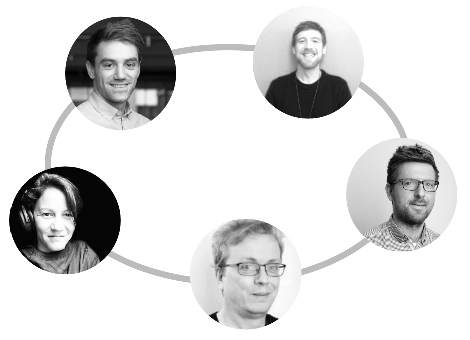
\includegraphics[width=\textwidth]{figures/group_photos.pdf}
\end{frame}

\begin{frame}[t]{Overview}
    \begin{enumerate}
        \item Background
            \begin{itemize}
                \item What's the problem?
                \item What solutions already exist?
            \end{itemize}
        \item Our approach
            \begin{itemize}
                \item Simulation to identify minimum sample size that satisfies criteria.
                \item Flexible, but slower.
                \item Gaussian process regression (via \texttt{mlpwr}) to speed up.
            \end{itemize}
        \item Next steps
    \end{enumerate}
\end{frame}

\section{Background}

\begin{frame}[t]{What's the problem?}

    Thousands of prediction models are developed every year.

    Prediction models can inform treatment decisions, facilitate screening, and
    enable stratified care.

    However, most are developed with inadequate samples:

    \begin{itemize}
        \item In a review of prediction models for COVID-19, the most frequent problem was insufficient sample size, with 67\% (408/731) of models developed on too few patients (Wynants et al., 2020).
        \item 56\% of models developed using supervised machine learning techniques are developed using inadequate sample sizes (Navarro et al., 2021).
        \item 73\% of prediction models for psychiatry had inadequate sample size (Meehan et al., 2022).
        \item Only 8\% of published machine learning models in oncology report a sample size justification.
    \end{itemize}
\end{frame}

\begin{frame}[t]{Inadequate samples $\rightarrow$ research waste}

    Inadequate samples lead to overfitting and inaccurate estimates of model
    parameters. Overfitting is where the model captures idiosyncrasies of the
    development sample, producing inflated estimates of predictive performance
    that cannot be replicated in the target population. Unreliable models may
    generate inappropriate decisions about patient care or lead to models not
    being implemented into clinical practice. Data collection can be invasive
    and inconvenient and diverts resources from other activities that benefit
    patients. Ensuring sample sizes are sufficient before model development
    would improve patient outcomes by avoiding models developed with inadequate
    samples and reducing participant burden.

\end{frame}

\begin{frame}[t]{Tools for estimating minimum sample sizes for prediction}

    Until recently, most studies ignored sample size.

    Or they used simple rules-of-thumb (e.g., 10 events per variable).

    In 2018, \texttt{pmsampsize} was released by Riley et al.

    \begin{columns}
        \begin{column}[c]{0.5\textwidth}
            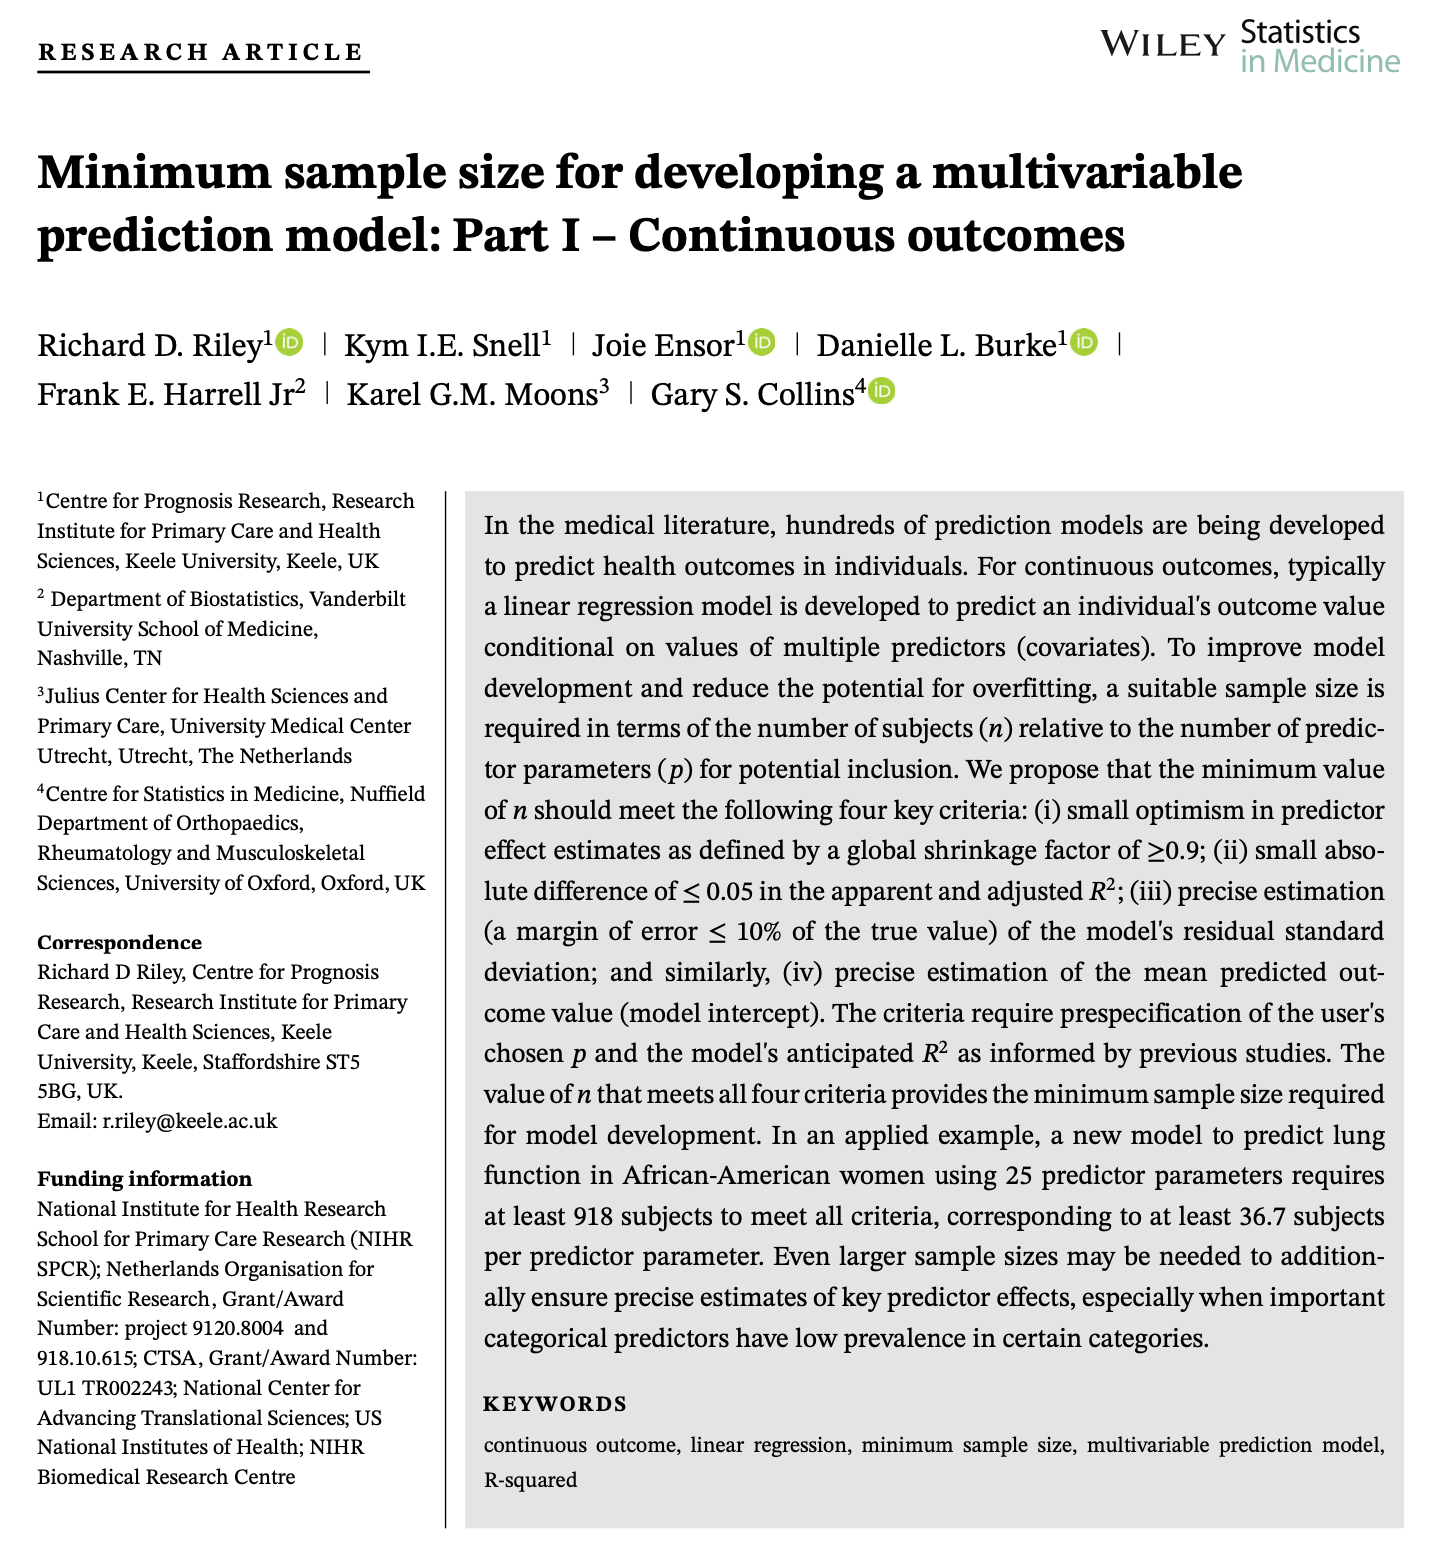
\includegraphics[width=\textwidth]{figures/riley1.png}
            	
        \end{column}
        \begin{column}[c]{0.5\textwidth}
            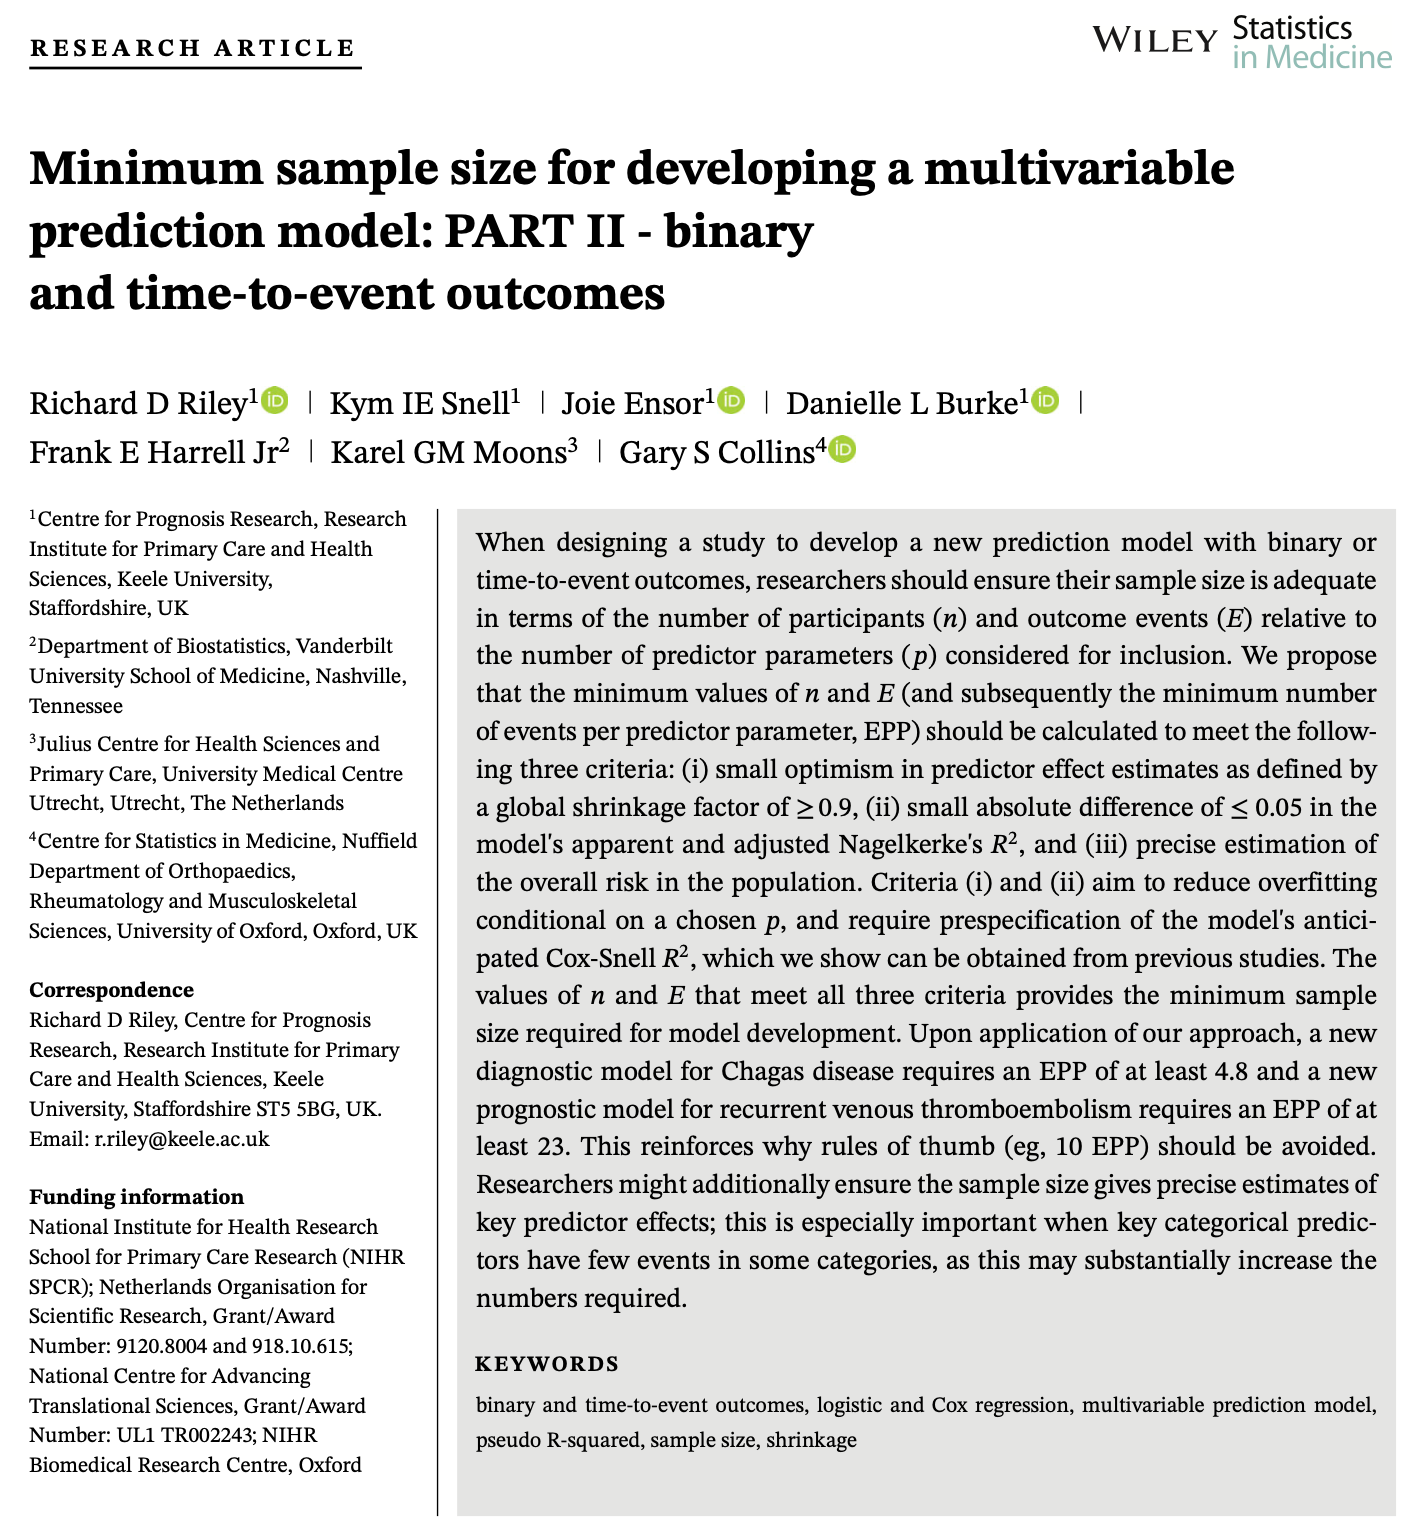
\includegraphics[width=\textwidth]{figures/riley2.png}
    
        \end{column}
    \end{columns}

\end{frame}

\begin{frame}{pmsampsize}

    The package identifies the minimum sample that results in: \\[1em]

    \centering

    \begin{tabular}{l>{\raggedright\arraybackslash}p{12em}>{\raggedright\arraybackslash}p{12em}}
        & \textbf{Continuous} & \textbf{Binary} \\ \midrule
        i.   & \multicolumn{2}{p{24em}}{Small optimism in predictor effect
        estimates, indicated by a global shrinkage factor of ≥ 0.9.} \\ \midrule
            ii. & \multicolumn{2}{p{20em}}{Small absolute difference of ≤ 0.05
            in the apparent and adjusted $R^2$} 	\\ \midrule
            iii.	& Precise estimation of the model's residual standard
            deviation. & Precise estimation of the overall risk in the
            population. \\ \midrule
            iv. & Precise estimation of the model intercept. & \\
    \end{tabular}

\end{frame}

\begin{frame}[t]{We \img{figures/heart.png} pmsampsize, however\ldots}

    pmsampsize has methods for simple continuous, binary, and survival outcome.

    However, we increasingly need to derive minimum samples for:

    \begin{itemize}
        \item Other model types, e.g., machine learning algorithms
            such as random forests or gradient boosting.
        \item Other data types, e.g., repeated measures and longitudinal data.
    \end{itemize}

    So, we've created a simulation-based framework for sample size estimation
    for prediction.

\end{frame}

\begin{frame}{pmsims}

    A simulation-based framework that derives the minimum sample that

    \begin{itemize}
        \item achieves with 10\% of the expected large-sample performance
        \item achieves calibration slope of >0.9
    \end{itemize}

    \begin{itemize}
        \item Any model or data type
        \item Defaults for common model/data types
        \item Fast(er).
    \end{itemize}

\end{frame}

\begin{frame}[c]{Our approach}

    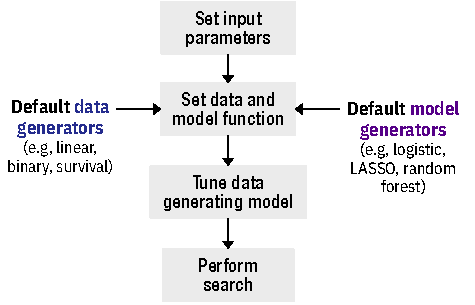
\includegraphics[width=\textwidth]{figures/workflow1.pdf}

\end{frame}

\begin{frame}[t]{Slide explaining input parameters and generators}

\end{frame}

\begin{frame}{Performing the search:\ \texttt{mlpwr}}

    A simulation-based approach with complex data/models would be too slow.

    mlpwr is a R package by 

    Felix Zimmer and Rudolf Debelak at the University of Zurich

     "A Power Analysis Toolbox to Find Cost-Efficient Study Designs"

\end{frame}

\begin{frame}[t]{Surrogate modeling}

    \begin{itemize}
        \item Surrogate modeling aims to approximate a relationship
            that is costly to investigate with a cheaper function
            (Bhosekar & Ierapetritou, 2018; Forrester & Keane,
            2009).

        \item  We can adopt the idea of surrogate modeling to the functional
            relationship between study design parameters and power.


        \item Using this functional relationship, we can predict the power for a
            sample size that we did not perform a simulation at beforehand.

        \item Surrogate modeling is more efficient than grid search: In a simple
            example, our approach required only 20\% of the computational effort and
            performed 50\% more simulation runs that used the optimal sample size
            (Zimmer \& Debelak, 2022).

            \end{itemize}

        \end{frame}

\begin{frame}[c]{Example}

    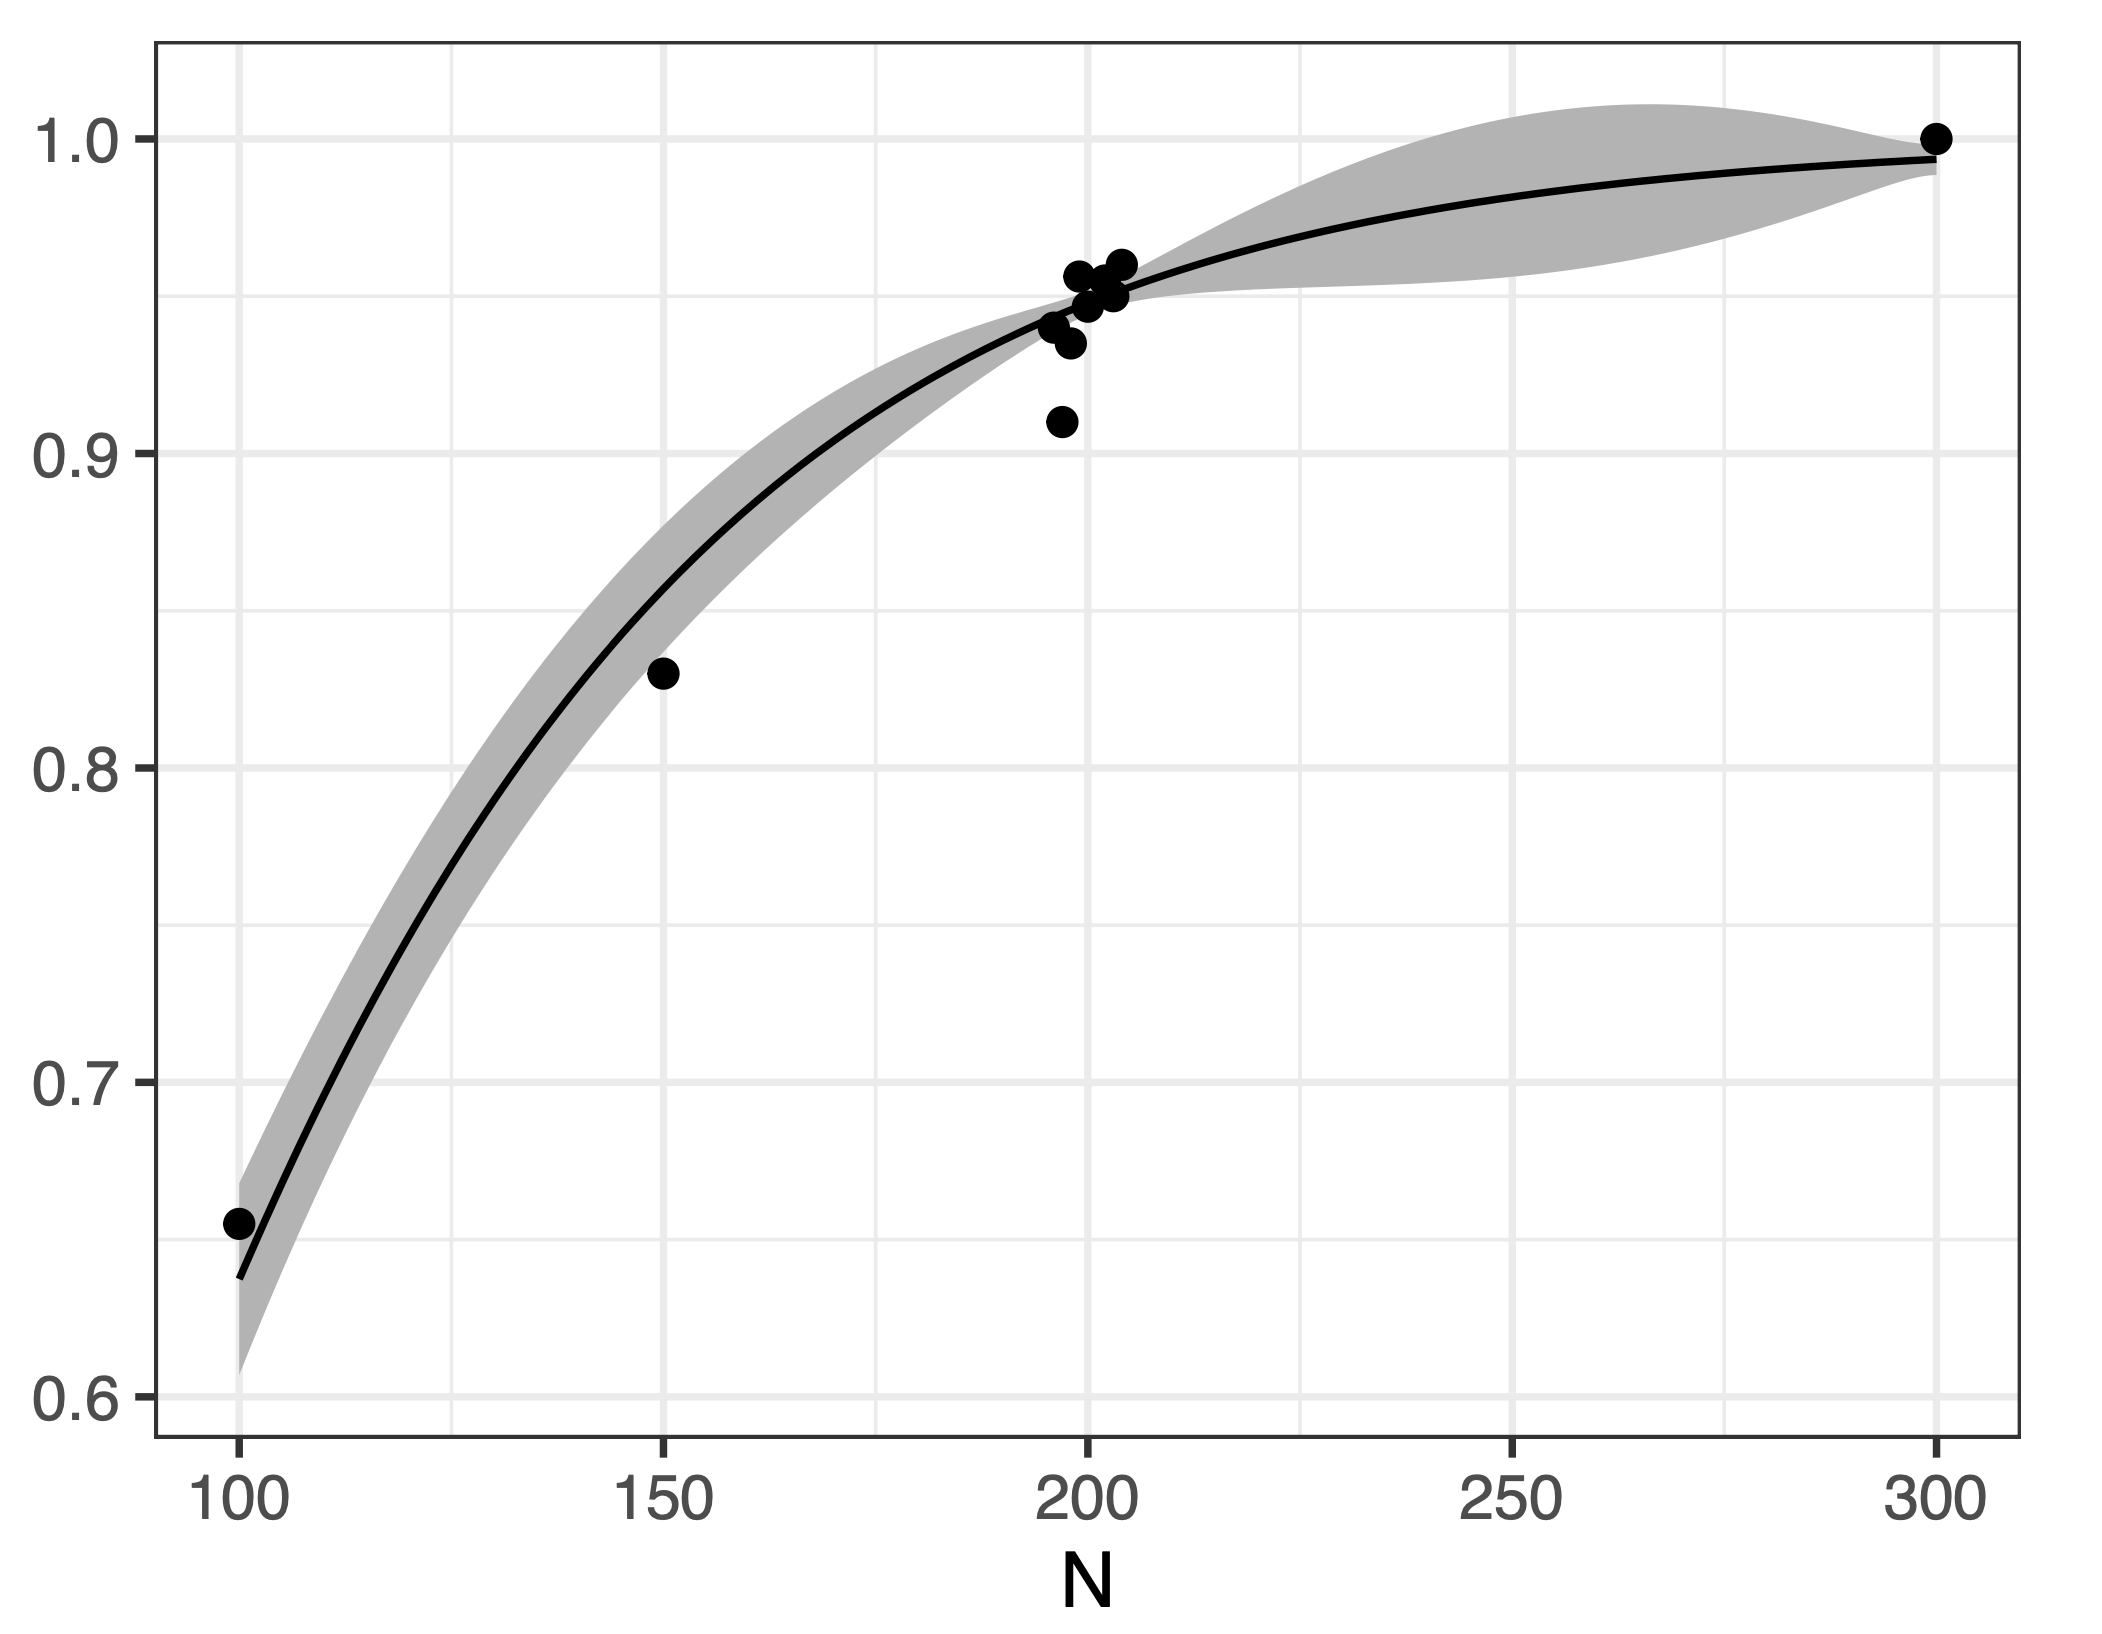
\includegraphics[width=\textwidth]{figures/mlpwr_example.png}

\end{frame}

\begin{frame}[t]{Slide explaining how we calculate the final sample size}

    The minimum sample that is within 10\% of expect large sample performance
    in 80\% of replications.

\end{frame}

\begin{frame}[t]{Example 1:\ Binary outcome, logistic regression }

\end{frame}

\begin{frame}[t]{Example 2:\ Linear outcome, XGBoost}

\end{frame}

\begin{frame}[t]{What's next?}

Package in development, functionining but more testing needed. Follow
\href{https://fediscience.org/@ewan}{fediscience.org/@ewan} for updates or LINK
TO SIGN-UP.

\begin{cbox}{KCLtealblue}{1.\ Machine learning}{}

\end{tcolorbox}

\begin{cbox}{KCLpurple}{2.\ Longitudinal data}{}

\end{tcolorbox}

\begin{cbox}{KCLhotpink}{3.\ Performance}{}

\end{tcolorbox}

\end{frame}

% For presentation: for example, a data with ~20 params and prevalence of 0.2 achieved performance of 0.75 AUC, We can then use our package to calculate sample size and compare with pmsampsize, Then, we use the tuned data generator from LR and check what is the performance for LR-Lasso and min sample size. Then, same for XGBoost. Riley seemed to advocate that XGBoost would need manifold more than LR, so we can check ![](20_f.png)

% Do it for ridge regression
% Do it for ML algorithms
% Then point to a mixed model.


\section{Conclusion}

\begin{frame}
  Questions?
\end{frame}

\appendix

\begin{frame}[fragile]{Backup slides}

\end{frame}

\begin{frame}[allowframebreaks]{References}
  \bibliography{demo}
  \bibliographystyle{abbrv}
\end{frame}

\end{document}
